\section{Implementation and Technologies}\label{sec:technology}

We have developed the Automated Journalist App using appropriate technologies. To meet our requirements, we needed a user-friendly application with a modern design, supported by a frontend framework that aligns with our design concept. In addition, before starting the project we had a codebase written in Python capable of generating summaries from given texts. Our objective was to extend this codebase, integrate it with a user interface, and transform it into a fully functional application. We carefully selected our technology stack to align with these goals.

Furthermore, we integrated two additional APIs into the application alongside the Twitter API. Specifically, we implemented connections to Reddit and Telegram, enabling us to use these platforms as additional data sources. 

The technologies we selected for this app are:
\begin{itemize}
    \item Backend: Python with Flask Framework
    \item Frontend: React with Typescript
    \item UI/UX design: Figma
\end{itemize}

The structure of the application is as in the following diagram (figure \ref{fig:architecture}). As illustrated in the figure, the Flask application serves as the bridge between the frontend, third-party social media APIs, and our AI models, which are used to summarize content from the social media feeds.

\begin{figure}
    \centering
    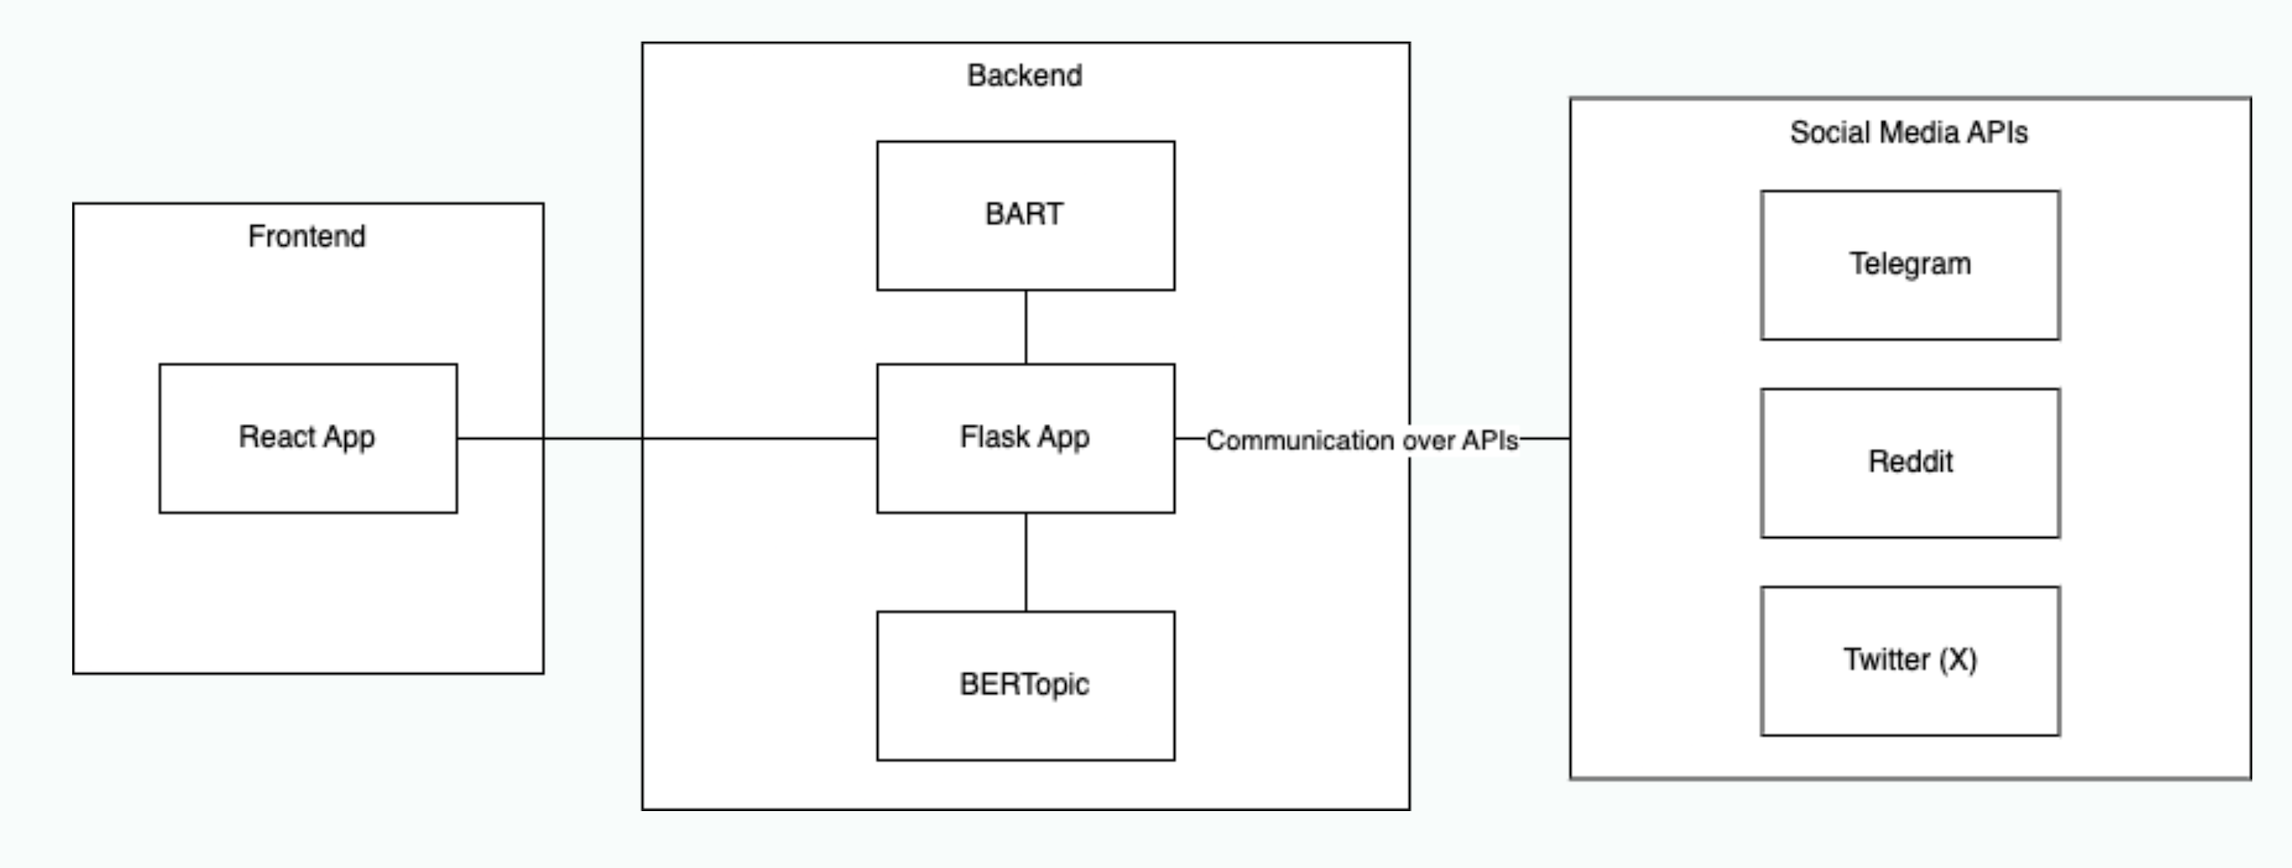
\includegraphics[width=\linewidth]{figures/general-architecture-of-the-app.png}
    \caption{Architecture of the App}
    \label{fig:architecture}
\end{figure}

\subsection{Backend}

As previously mentioned, at the outset of the project, we had a Python codebase as our starting point. We extended this code to develop the project into a fully functional application. Python was also chosen due to its extensive libraries, which are particularly advantageous in the fields of machine learning and natural language processing.\citep{ml-python}

Moreover, Python offers several libraries that facilitate the integration of third-party applications through their APIs. Relevant examples include Twat for Twitter, PRAW for Reddit, and Telethon for Telegram.

The backend application functions as a REST API endpoint for the frontend, and it is built using Python Flask. This Flask application consolidates calls to third-party APIs and integrates them with the NLP models we use for generating summaries. The application does not include any authentication or authorization mechanisms. The social media feeds obtained from the sources are not personalized; rather, they are retrieved by querying these platforms through the API endpoints maintained and published by the respective social media providers. At the backend application, we implemented some endpoints only retrieving data from the respective social media platforms.

Additionally, we have implemented endpoints to process summaries from the feeds selected by the user. Our application offers three distinct summarization functionalities: "Default Summary," "Topic-Aware Summary," and "Delta Summary."
\begin{itemize}
    \item The Default Summary provides a summary of the selected feed.
    \item The Topic-Aware Summary generates potential topics from the default summary and then produces summaries of the same feed, tailored to those identified topics.
    \item The Delta Summary allows users to compare summaries across different topics, enabling them to see how divergent the summaries are within various topic perspectives.
\end{itemize}

Details on the specific implementation of these functionalities, including the models used, will be provided in the section \ref{sec:summarization} "Summarization Techniques".

\subsection{Frontend}
To enable access to the application's functionalities, we have implemented a web-based user interface. For the user interface, we utilized the React framework with TypeScript, which provided the advantage of using hooks to create a more responsive application with improved communication between the frontend and backend. While implementing the application, we have tried to utilize the principles of Object Oriented Programming.

Before writing any code, we first created a design concept using Figma. Once the concept was established, we began coding. During the development process, we made extensive use of the React library Material-UI to align the implementation with our design as closely as possible.

\subsection{Samsum Dataset Format}\label{subsec:samsum}

In our application, we retrieve data from various social media providers and needed to standardize this data into a uniform format. This standardization ensures that our summarization implementation can effectively process and summarize data across different social media platforms. To achieve that goal, we utilized the "Samsum Dataset Format" which was introduced by \cite{samsum}. We fetched that data from the social media and transformed the data with the following schema:
\begin{itemize}
    \item dialogue: text of dialogue.
    \item summary: human written summary of the dialogue.
    \item id: unique id of an example.
\end{itemize}

We have also utilized this format as an interface between the backend and frontend. The application fetches data from a social media platform and sends it to the frontend as in the defined "samsum" format. The social media feed is then displayed accordingly. When a user wishes to summarize a feed, they select the feed by clicking on it. The selected feed is then transmitted in the "samsum" format to the backend, where it is summarized. This methodology streamlines the process of handling data from different sources, as it eliminates the need to format each source individually. Moreover, if there is a need to integrate additional data sources, the same methodology can be employed. The new feed can be converted to the "samsum" format, allowing the existing functionalities to be applied seamlessly.
 
\subsection{How does the application work?}\label{subsec:how_app_work}
This subsection outlines how the application functions from a user's perspective. We will explore the actual use cases of the application, accompanied by real in-app screenshots, to provide a clearer understanding of how the app operates. The in-app screenshots are given at the end of the report in Appendix \ref{sec:appendix}.

The application does not include any authorization or authentication mechanisms as also stated above. As a result, when the user accesses the home page, they can immediately begin using the application's functionalities without the need for any additional steps.

The home page of the application greets the user with a search bar, allowing them to perform queries within social media platforms. Above the search bar, there are tabs where the user can select the specific social media provider from which the query will be issued. The screenshot of the displayed figure has been given in the Appendix as the figure~\ref{fig:home_page}.

Once the feeds are fetched from the social media, they are displayed to the user. A feed is a set of data that is structured as in the samsum dataset format as also described in the subsection "Samsum Dataset Format" (Section \ref{subsec:samsum}). Some conversations in the social media have been displayed to the user as in the figure \ref{fig:home_page}

The user then selects one of these conversations, which is sent to the backend for summarization. Upon completion of the summarization task, the "Default Summary" is returned and displayed to the user. Simultaneously, the "Topic-Aware Summary" is processed, along with the associated topics. These topics are also presented in the user interface. To view summaries related to each specific topic, the user can select the desired topics from a drop-down menu located at the top right of the display, as shown in the figure \ref{fig:summary_default}.

Subsequently, the user selects a topic from the drop-down menu, and the summary related to that topic is displayed (see figure \ref{fig:summary_topic_options}). Additionally, the user can compare summaries across different topics to assess how they differ from one another. To utilize this functionality, the user clicks the "Compare Summaries" button, which opens a selection popup. The user then selects the topics to be compared.(figure \ref{fig:compare-summaries})

Once the topics are selected, these choices are transmitted to the backend to generate the "Delta Summary." The results of the "Delta Summary" are presented in two visualization formats: a scatter plot (figure \ref{fig:delta-summary-scatter}) and a cosine similarity matrix (figure \ref{fig:delta-summary-cosine}).